This study adopts a structured artificial intelligence pipeline to develop a decision support system for agricultural skill development. The overall framework integrates data preprocessing, segmentation, predictive modeling, and explainable analysis into a unified workflow.

\subsection{Data and Study Context}

The dataset consists of panel survey data collected from farmers participating in the Smart Farmer program in Thailand. Observations include pre-training and post-training measurements, capturing demographic characteristics, resource access, risk perception, and multiple dimensions of agricultural skills. The primary outcome variable is the change in overall skill score, denoted as $Ch\_Skill$, defined as the difference between post-training and pre-training composite scores.

Missing values in the dataset were handled using simple imputation strategies. Binary and asset-related variables were imputed with zero, while continuous variables were imputed using mean values. All numeric variables were standardized prior to modeling to ensure comparability across features.

\subsection{Farmer Segmentation}

Farmer heterogeneity was addressed using K-Means clustering. The clustering process was applied to baseline features including skill scores, demographic characteristics, and risk indicators. The Euclidean distance metric was used to measure similarity between observations in the standardized feature space.

The number of clusters was determined based on the combined use of the Elbow method and Silhouette analysis\cite{rouseeuw1987}. The resulting clusters represent distinct farmer segments characterized by different levels of baseline capability and resource constraints. These segments form the first stage of the decision support system.

\subsection{Predictive Modeling}

A Random Forest regression model was employed to predict skill improvement outcomes\cite{breiman2001}. The model was trained using features related to farmer characteristics, baseline skills, and risk perception. Model performance was evaluated using cross-validation, with the coefficient of determination ($R^2$) used as the primary metric.

In addition, XGBoost was tested as a robustness check to ensure consistency of predictive performance across model types. The results indicate comparable performance between the two models, supporting the reliability of the predictive component \cite{chen2016}.

\subsection{Explainable AI Analysis}

To ensure interpretability, SHapley Additive exPlanations (SHAP) were applied to the trained model. SHAP values provide a consistent measure of feature contribution to each prediction, allowing both global and local interpretation of model behavior.

Global feature importance was derived using mean absolute SHAP values, while SHAP summary plots were used to visualize the distribution and direction of feature effects. In addition, SHAP analysis was conducted at the cluster level to identify segment-specific drivers of skill improvement.

\subsection{Decision Support Framework}

The proposed decision support system follows a three-stage architecture: Segment, Attribute, and Recommend (fig~\ref{fig:framework}).

In the first stage, farmers are assigned to segments using clustering results. In the second stage, SHAP values are used to identify the most influential factors within each segment. In the final stage, these insights are translated into explicit decision rules that guide training allocation.

This framework enables the transformation of machine learning outputs into actionable recommendations, supporting real-world implementation in agricultural extension systems.

\begin{figure}[t]
\centering
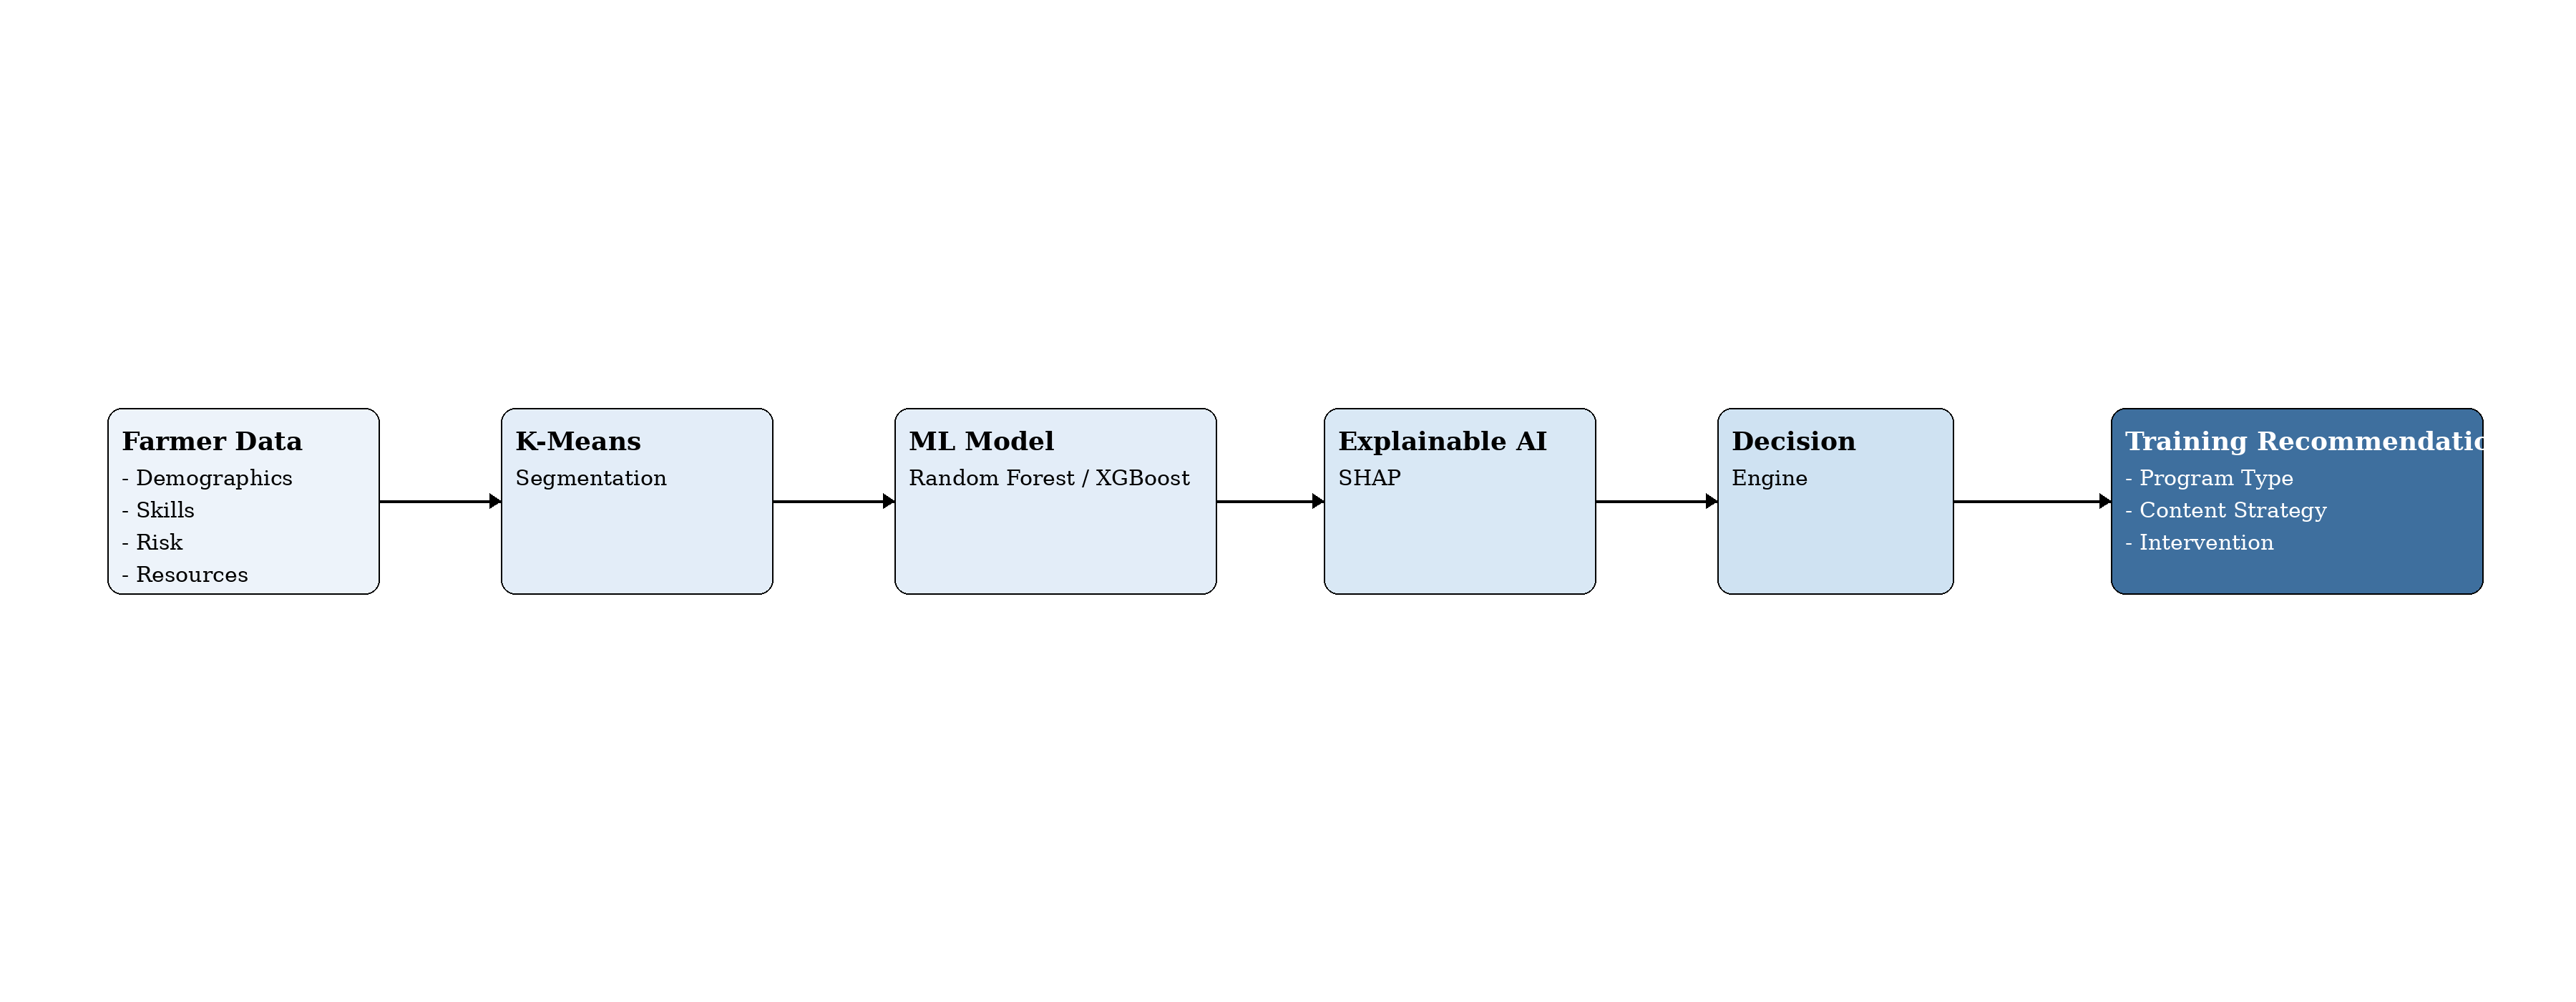
\includegraphics[width=\columnwidth]{figures/fig1_framework.png}
\caption{The proposed explainable AI-based decision support framework integrating segmentation, predictive modeling, and SHAP-based explanation within a Segment--Attribute--Recommend pipeline.}
\label{fig:framework}
\end{figure}